\documentclass[border=2mm,
               tikz,
               preview]{standalone}
\usetikzlibrary{positioning,chains}

\begin{document}

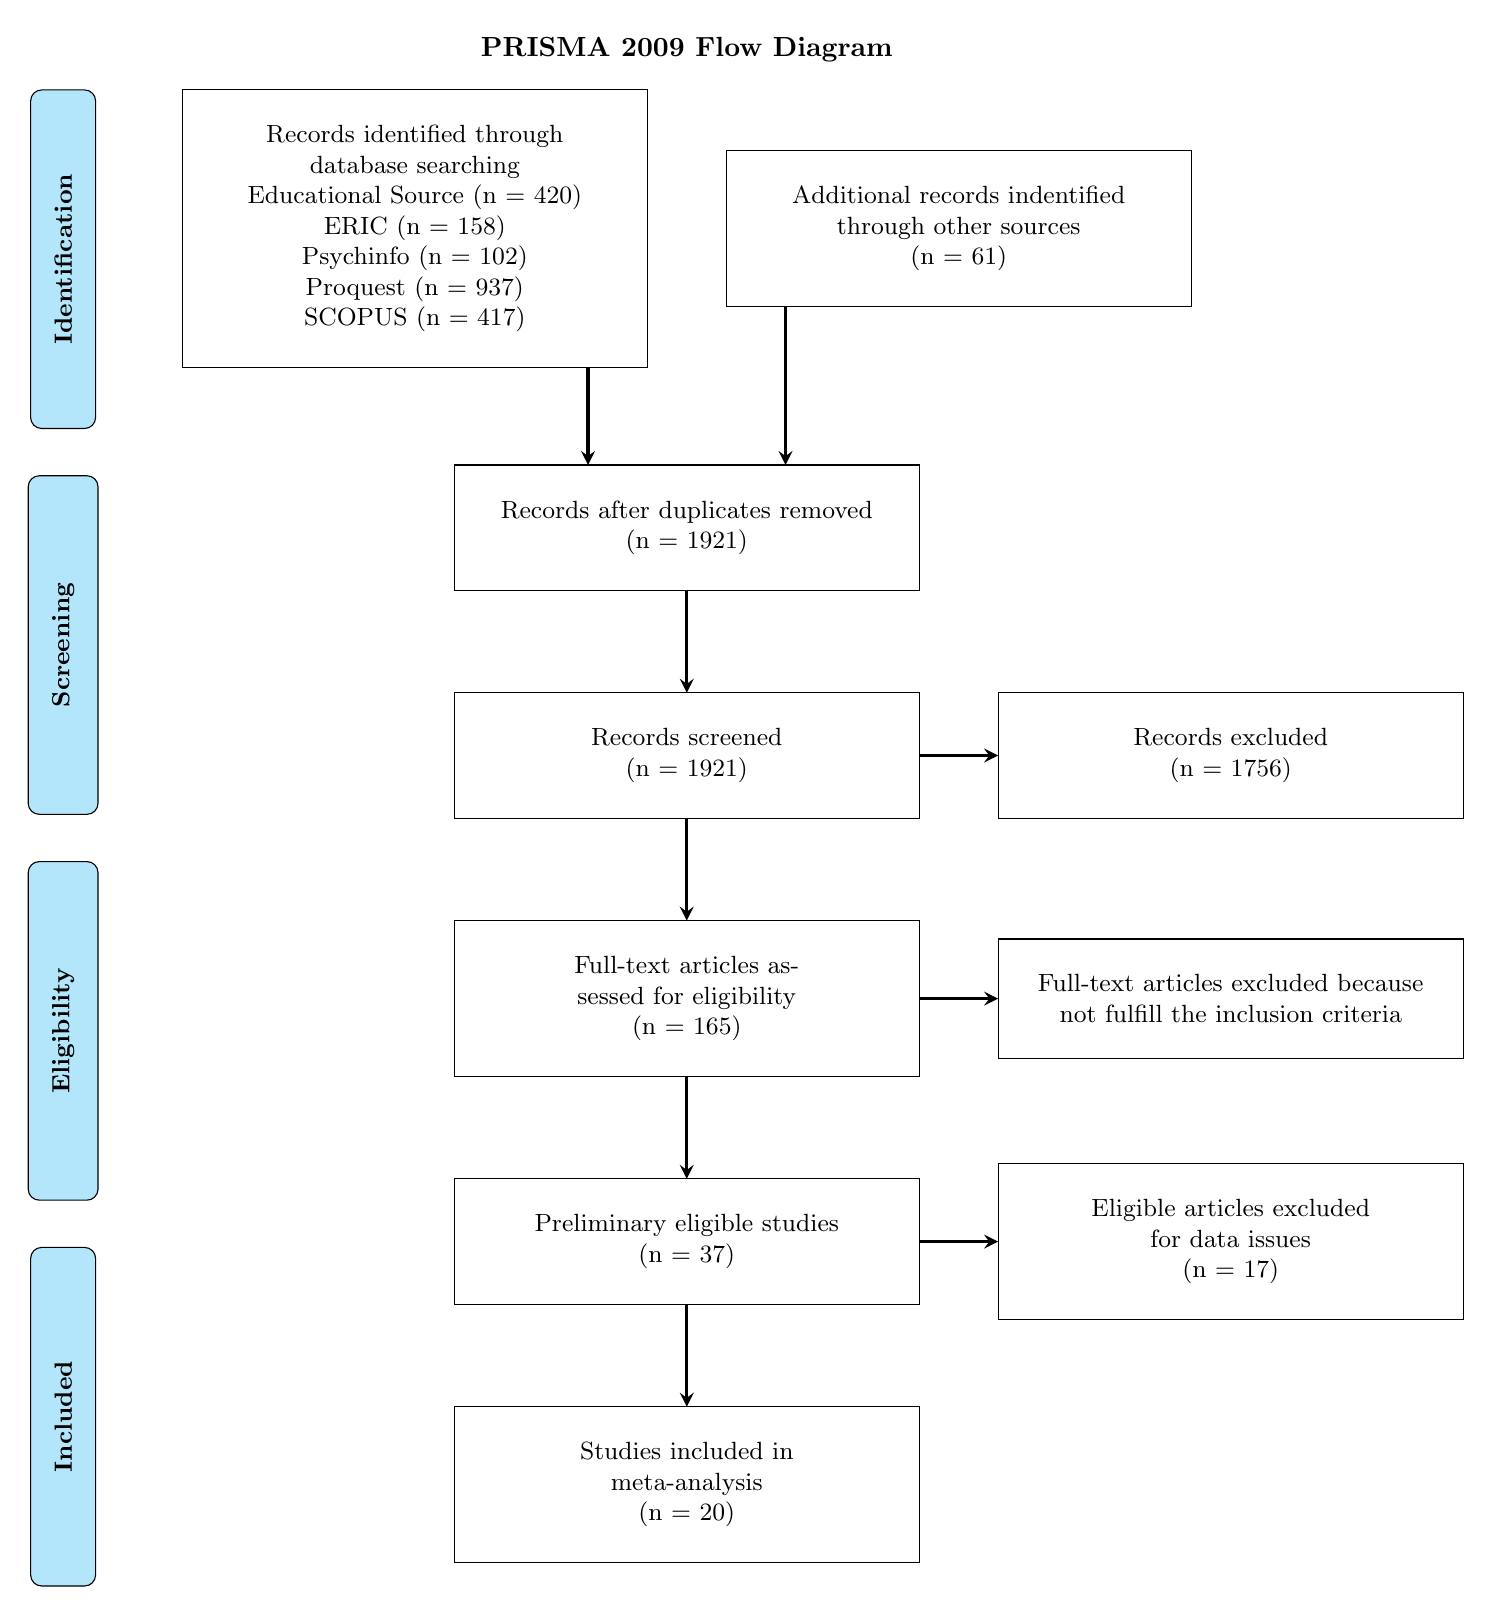
\begin{tikzpicture}[
    node distance=13mm and 10mm,
    start chain=going below,
 mynode/.style = {
        draw, rectangle, align=center, text width=5cm,
        font=\small, inner sep=3ex, outer sep=0pt,
        on chain},
mylabel/.style = {
        draw, rectangle, align=center, rounded corners, 
        font=\small\bfseries, inner sep=2ex, outer sep=0pt,
        fill=cyan!30, minimum height=43mm,
        on chain},
every join/.style = arrow,
     arrow/.style = {very thick,-stealth}
                    ] 
\coordinate (tc);
% the title
\node[above= 2 cm of tc,font=\bfseries] {PRISMA 2009 Flow Diagram};
% the nodes at the top
\node (n1a) [mynode, left= 5 mm of tc]    {
Records identified through database searching\\
                                    Educational Source (n = 420)\\
                                    ERIC (n = 158)\\
                                    Psychinfo (n = 102)\\
                                    Proquest (n = 937)\\
                                    SCOPUS (n =  417)
                                    };
\node (n1b) [mynode,right= 5 mm of tc]    {Additional records indentified\\
                                        through other sources\\
                                        (n = 61)};
    % the chain in the center
\node (n2)  [mynode, below= 3 cm of tc]   {Records after duplicates removed\\
                                      (n = 1921)};
\node (n3)  [mynode,join]   {Records screened\\
                            (n = 1921)};
\node (n4)  [mynode,join]   {Full-text articles assessed for eligibility\\
                            (n = 165)};
\node (n5)  [mynode,join]   {Preliminary eligible studies\\ 
                            (n = 37)};
\node (n6)  [mynode,join]   {Studies included in\\ meta-analysis\\
                            (n = 20)};
% the branches to the right
\node (n3r) [mynode,right=of n3]    {Records excluded\\
                                    (n = 1756)};
\node (n4r) [mynode,right=of n4]    {Full-text articles excluded because not fulfill the inclusion criteria};
\node (n5r) [mynode,right=of n5]    {Eligible articles excluded\\ for data issues\\
                                    (n = 17)};
% lines not included in join                                        
\draw[arrow] ([xshift=+22mm] n1a.south) coordinate (a)
                                       -- (a |- n2.north);
\draw[arrow] ([xshift=-22mm] n1b.south) coordinate (b)
                                       -- (b |- n2.north);
\draw[arrow] (n3) -- (n3r);
\draw[arrow] (n4) -- (n4r);
\draw[arrow] (n5) -- (n5r);

% the labels on the left
    \begin{scope}[node distance=6mm]
\node[mylabel,below left=0mm and 11mm of n1a.north west]
                {\rotatebox{90}{Identification}};
\node[mylabel]  {\rotatebox{90}{Screening}};
\node[mylabel]  {\rotatebox{90}{Eligibility}};
\node[mylabel]  {\rotatebox{90}{Included}};
    \end{scope}
\end{tikzpicture}
\end{document}